In Section~\ref{section:rational-numbers} we've seen that almost all rational numbers $q \in \mathbb{Q}$ determine a finite cover $q\colon\Spec(\mathbb{Z}) \mapsto \mathbb{P}^1 / \mathbb{F}_1$, the exceptional cases controlled by \href{http://en.wikipedia.org/wiki/Zsigmondy's_theorem}{Zsigmondy's theorem}.

The prime exceptional case corresponds to $q=2$. Below,we sketch a small portion of the graph of this non-cover (the image does not contain the points $[1]$ and $[6]$, the red lines) where we use a logarithmic scale on $\Spec(\mathbb{Z})$.

\begin{figure}[ht]
  \centering
  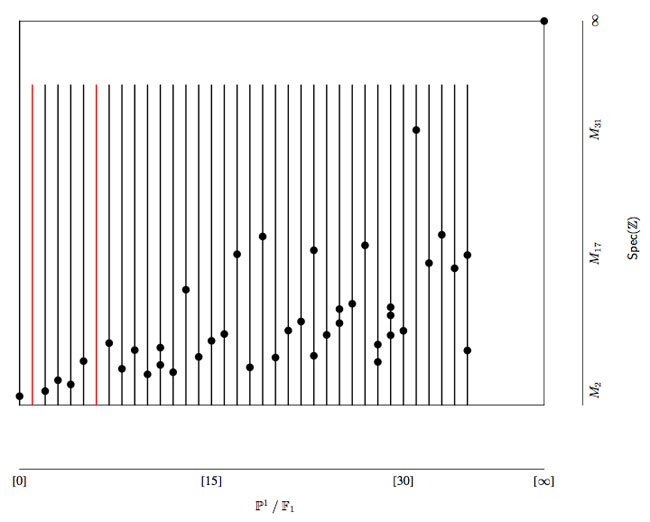
\includegraphics[width=11cm]{exceptional-map/mersenne.jpg}
  \caption{Impression of the exceptional map~$q=2$}
  \label{figure:mersenne}
\end{figure}

Clearly, such images should be taken with a bucket of salt. The linear depiction of $\Spec(\mathbb{Z})$ suggests for example that the prime $3$ has more affinity with $2$ and $5$ than with say $2147483647$ or $524287$. However, the relevant topology on $\Spec(\mathbb{Z})$ is the cofinite topology, so one is always allowed to reshuffle finitely many primes in order to get a smoother covering  map!

The fiber over $[n]$ consists of the primitive prime factors of $2^n-1$ (that is, those primes not dividing $2^d-1$ for $d$ a proper divisor of $n$). For small values of $n$, most fibers consist of just one prime (for $n \leq 35$ only $n=11,23,23,28$ and $35$ have two principal primes and only $n=29$ has three primes in its fiber).

A \href{http://en.wikipedia.org/wiki/Mersenne_prime}{Mersenne prime} is a prime number of the form $\mathrm{M}_p = 2^p-1$ (from which it follows that $p$ must be prime, too). Only $47$ Mersenne primes are known, the smallest being
\begin{equation}
  \mathrm{M}_2,\mathrm{M}_3,\mathrm{M}_5,\mathrm{M}_7,\mathrm{M}_{13},\mathrm{M}_{17},\mathrm{M}_{19}\text{ and }\mathrm{M}_{31}
\end{equation}
corresponding to the points on 'the diagonal' in the graph of the exceptional map. Naturally, if $\mathrm{M}_p$ is a Mersenne prime, the fiber $2^{-1}([p])$ has only one element.

If we believe a geometry over $\mathbb{F}_1$ can be developed such that the morphisms $q$ make sense (and hence their graphs define divisors in the Smirnov plane $\Spec(\mathbb{Z}) \times \mathbb{P}^1 / \mathbb{F}_1$) one might expect that the subsets of points $[n] \in \mathbb{P}^1 / \mathbb{F}_1$ with a fiber containing at least $k$ points, should be cofinite.

In particular, in view of Schinzel's result (stating that all maps $q$ have infinitely many points with a fiber containing at least two elements) this would imply that the set of Mersenne primes has to be finite, contradicting the \href{http://en.wikipedia.org/wiki/Lenstra-Pomerance-Wagstaff_conjecture}{Lenstra-Pomerance-Wagstaff conjecture}.

On the positive side, it would imply that infinitely many numbers of the form $2^p-1$ (with $p$ a prime number) are highly composite (as they must have at least two principal prime factors) which is another big open problem\ldots
